\begin{figure*}[t]
\centering
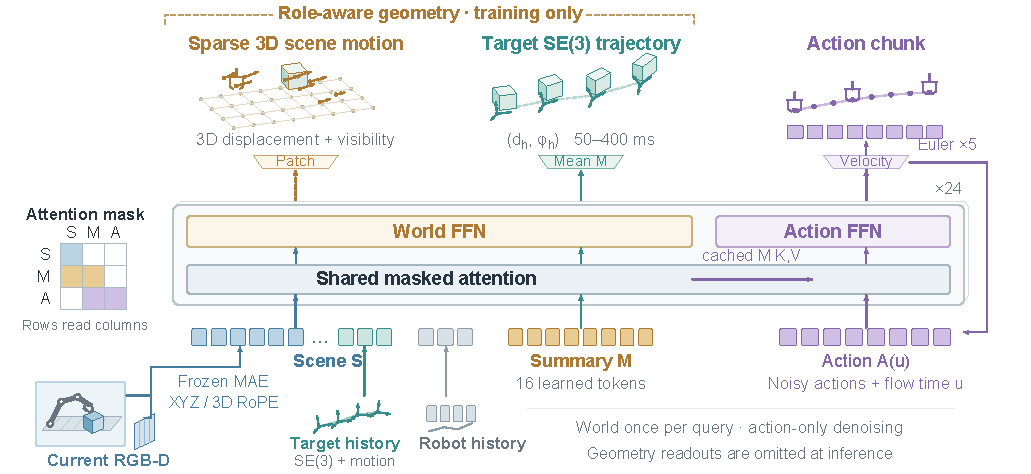
\includegraphics[width=\textwidth]{figures/Fig2/fig2_se3wam.pdf}
\caption{\textbf{\ours 架构。}自下而上阅读。当前 RGB-D、目标历史（蓝色坐标轴）和机器人历史组成 $S=212$ 个场景 token。单一主干共享掩码注意力，使用分流 FFN；动作读取 16 个摘要 token $M$。虚线框仅用于训练：patch 状态接受全场景稀疏 3D 流及可见性监督，摘要均值接受目标 SE(3) 轨迹监督。图中几何画面来自同一条 \bench{} 传送带轨迹的真实标签：左侧显示 $14\times14$ 网格在 400\,ms 的工作区裁剪，橙色坐标轴对应未来 50--400\,ms 的八个位姿。紫色路径为专家轨迹中记录的末端执行器状态，用于说明动作空间，不是策略预测。RGB 场景画面由记录状态经 Blender 渲染。推理时跳过整个虚线框，世界流键值在 \cfgEuler{} 个动作 Euler 步中复用。}
\label{fig:architecture}
\end{figure*}
